\documentclass[12pt]{ctexart}

\usepackage{graphicx}
\usepackage[hmargin=1.1in,vmargin=1in]{geometry}
\usepackage{indentfirst}
\usepackage{multirow}
\usepackage{makecell}
\usepackage{gbt7714}
\usepackage[defaultmono,scale=0.85]{droidsansmono}
\usepackage[colorlinks=true]{hyperref}

\bibliographystyle{gbt7714-numerical}

\fontsize{14pt}{1.0}

\newlength{\blanklength}
\setlength{\blanklength}{40ex}

\providecommand{\thetitle}{对华为``寒风''的分析与思考}
\providecommand{\theauthor}{Sparky\_14145}
\providecommand{\thestudentID}{71XXXXXX}
\providecommand{\theemail}{Sparky\_14145@outlook.com}
\providecommand{\theinstitution}{College of Software Engineering}

\input{personal_info/info.tex}

\providecommand{\blankToFill}[1]{
    \parbox[t][3ex]{\blanklength}{
        \makebox[\blanklength]{#1}\\[0pt]
        \rule[2ex]{\blanklength}{0.1ex}
    }
}

\providecommand{\makecover}{\begin{titlepage}
    \noindent
    {东南大学} \\[2pt]
    {\Large \bfseries 课程报告}

    \vspace*{20pt}
    \begin{center}
    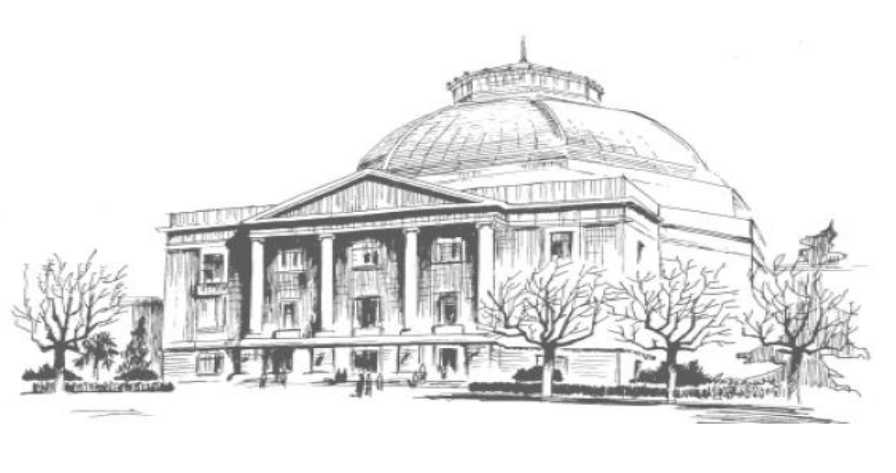
\includegraphics[width=0.8\textwidth]{pics/cover.png} \\
        \textsc{\Huge 经济管理基础} \\[2pt]
        \textsc{\huge 课程报告}

        \vspace*{10pt}
        \begin{tabular}[c]{rc}
            题目        & \blankToFill{\thetitle} \\
            日期        & \blankToFill{\today} \\
            姓名        & \blankToFill{\theauthor\footnotemark} \\
            学号        & \blankToFill{\thestudentID} \\
            学院        & \blankToFill{\theinstitution} 
        \end{tabular}
        \rmfamily
    \end{center}

    \vspace*{0pt}
    % \begin{abstract}
    % \end{abstract}
    \footnotetext{\theemail}
\end{titlepage}}

\begin{document}
    \makecover

    \tableofcontents
    \newpage

    8 月 22 日下午,华为内部论坛上线了一篇关于《整个公司的经营方针要从追求规模转向追求利润和现金流》的文章\cite{start},其中的内容,特别是``把寒气传递给每一个人'',引发了广大网友的激烈讨论。即使是到笔者写下本文时(11 月),笔者仍能在许多应届毕业学长学姐那里听到``寒气''这两个字。于是,笔者写下本文,尝试分析``寒气''的由来,以及为何能够引发如此广泛的讨论。

    \section{从``为理想奋斗''到``努力活下去''}

    8 月 22 日,任正非在华为内部发出``寒气''文,通告公司的员工,公司正处于危急之中,并发出了接下来几年应当如何经营各项业务的``命令''。

    由于并没能搜索到华为``寒气''文的原文,笔者阅读了第一财经整理的任正非主要观点,发现主要包含以下几点内容:\cite{origin}

    \begin{enumerate}
        \item 盲目投资的业务要收缩。具体来说就是要控制开支,减少或关停竞争力不强的业务所导致的开支;
        \item 放弃部分市场。与第一点类似,控制开支,减少或关闭``挣不到钱''的市场上的投入;
        \item 让寒气传递到每个人。简单来说就是提高工资差距,刺激员工更加努力地创造现金流;
        \item 生存危机点上不惜代价投入。强调重视质量,在质量上多投入,避免因质量导致丢失市场。
    \end{enumerate}

    纵览全文,笔者注意到一件事情,那就是任老似乎一直在强调一件事:现在公司不是在``为理想奋斗'',不是要``为全人类服务'',而是要``活下来'',有质量地``活下来''。理想?理想就是活下来。为了活下来,任老甚至说出了``哪里有钱就在哪里赚一点''这种俗气却真实的话。为了让公司``活下来'',``公司是我家''这种话术任老不再使用,反而是很冰冷地告诉大家``奖金不是公司给的,是军团自己挣来的利润,而且还交给公司一部分''。也许正是这冷冰冰而又现实的话语,加上``还交给公司一部分''这种``路灯挂件''发言,导致了网络上的疯狂转发与讨论。

    不少人讨论``寒气''文,应该有一个原因,就是怀疑任老是想假借寒气的名义,行剥削员工之实,而所谓``寒风''可能并不透骨冰寒,甚至可能只是让人觉得凉爽。他们的观点正确吗?通过查阅华为 2021 年年报\cite{annual-2021},笔者了解到,``寒气''也许并非任老随口捏造出来的。

    华为 2021 年的销售收入为 636,807 万元,在近五年中排第二。如果只考虑销售收入,可以发现,华为的``业绩''在疫情爆发的 2020 年都没有下降,反而是在 2021 年跌到了只比四年前高一点。

    \begin{figure}[hp]
        \centering
        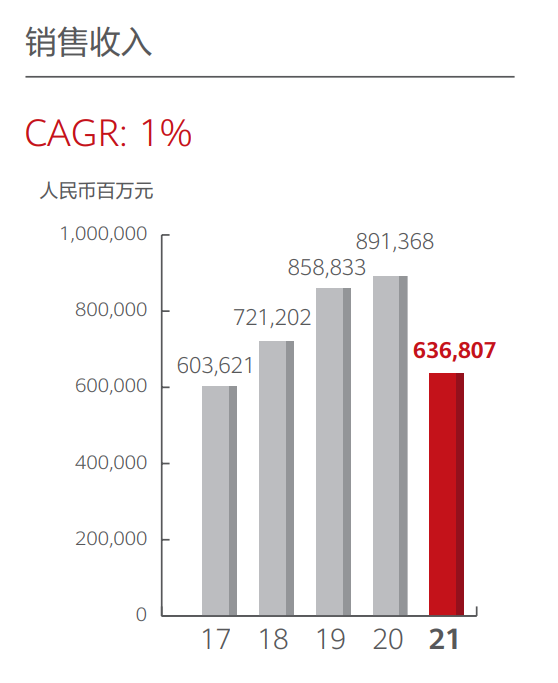
\includegraphics[width=0.5\textwidth]{pics/2021-sell-income.png}
    \end{figure}

    而即便是在销售收入大幅度下滑的情况下,华为依然大幅度提高了投资活动使用的现金流量净额\cite{annual-2021},这就使得华为 2021 年实际上处于亏损状态,尽管 2021 年华为减少员工工资支出与向雇员的支出约 30\%,却并没有改变这个状态。

    再进一步查看,发现 2021 年华为收入分部中,下降比例和数额最大的部分是消费者业务,笔者推测此部分业务应该主要与智能手机等项目相关,也就是受到美国政府相关政策影响较大的一部分。

    同时,笔者也查看了与华为公司有相似业务的,小米公司的年报与半年报。小米的利润在 2021 年与 2022 年上半年都处于增长之中,但是智能手机的毛利也有 30\% 到 50\% 的下跌。并且根据分地区的结果来看,这些下跌是全球性的。

    综合上述内容来看,所谓``寒气''并非危言耸听,而是智能手机行业确在经历着一些事情。

    \newpage
    \section{对``寒气''的思考}

    从经济学上来看,任老的主要观点,是符合经济学原理的:

    \begin{enumerate}
        \item 盲目投资的业务要收缩:降低那些 $MR < MC$ 以及 $MR - MC$ 较小的业务,以将更多的成本投入到 $MR - MC$ 较大的业务中获利;
        \item 放弃部分市场:退出那些 $P - ATC$ 较小的甚至小于 0 的市场,同样是为了将一部分产量投入到 $P - ATC$ 较大的市场中去提高获利;
        \item 让寒气传递到每个人:减少固定工资,降低企业的固定成本(?),并同时利用收入效应降低员工能负担的物品量,增加劳动供给量;然后提高奖金,利用替代效应,令闲暇相对于劳动更加昂贵,刺激员工减少闲暇时间增加劳动供给量;
        \item 生存危机点上不惜代价投入:使产品成为``高档物品''。
    \end{enumerate}
    \nocite{*}
    \bibliography{citations}
\end{document}